\section{MATERIALS AND METHODS}

\subsection{Experimental Design}

The study evaluates tool-mediated grounding through four experiment families: toolpath generation on ten anchor designs, orchestration on two stock variants of each design, language-model interfaces, and an external audit of the removal verifier. Only the work-order comparison pairs contract calls and free-form scripts on the same twenty instructions using Qwen3-8B. The instruction text and geometry backend are shared, but system prompts, interface documentation and output formats differ; the default output limits are 800 tokens for calls and 1,200 for scripts. The contract prompt additionally specifies the coordinate origin and subtractive semantics. This is a comparison of implemented interface packages, not an isolated causal intervention on action space. Direct numerical control generation uses ten different anchor-part tasks. The fifteen-model study compares models within the contract interface; it does not cross all models with all action spaces.

The original result ledger combines recomputed deterministic experiments with archived model and external-audit measurements. Revision audits read those archives without replacing them and record input hashes. The endpoint-lifting diagnostic, the audit of reference construction and the paired reanalysis are post hoc; none is presented as preregistered. Pass counts are reported as $k/n$. We distinguish finite-sample descriptions from generalisation claims, and do not combine different task families into a single success rate.

\subsection{Task Definition and Acceptance Criterion}

Given a part $P$ represented as a triangulated solid with face-level feature labels, a material grade $m$ and a stock allowance, the system must emit a restricted numerical control program $G$. Let $S(G)$ be the material left after executing $G$ in simulation. We accept $G$ only if

\begin{equation} \label{eq:accept}
\mathrm{gouge}_{\max}(S,P) \le 0.5\ \mathrm{mm}
\quad \mathrm{and} \quad
\overline{|S-P|} \le 0.5\ \mathrm{mm}.
\end{equation}

The first inequality limits irreversible excess removal in the discrete model. The second bounds average absolute error over represented target columns. Absolute errors do not cancel, but a small region with large error can be diluted by many accurate columns. These application-defined thresholds are not a dimensional-tolerance standard: local residuals can exceed 0.5 mm, and columns outside the rasterised target mask are not checked. We therefore retain worst-case and residual-volume diagnostics alongside acceptance. Equation~\ref{eq:accept} is an internal simulation criterion, not certification of a manufactured part.

\subsection{System Overview}

Figure~\ref{fig:1} shows the arrangement. The upper path is a four-stage pipeline: part input, spatial modality, manufacturing modality and verification. The lower path is an orchestration layer that observes the pipeline, records decisions and can send a failed plan back for a bounded retry. The gateway exposes tools through a Model Context Protocol server \cite{Anthropic2024MCP}; thirteen tools carry JSON schemas with geometric preconditions, and each call executes inside a snapshot transaction so that a failed call leaves no side effects. Seven error classes are intercepted at the boundary. FreeCAD 1.1.4 is the reference geometry kernel \cite{FreeCAD2025}.

\begin{figure}[htbp]
  \centering
  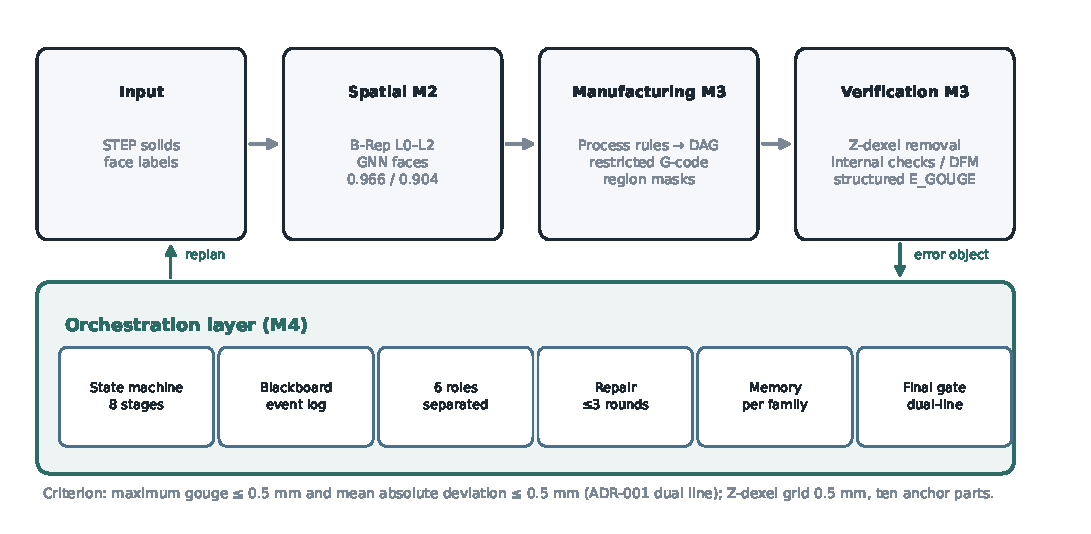
\includegraphics[width=\textwidth]{fig1.pdf}
  \caption{System overview. The upper path runs from part input through spatial and manufacturing modalities to verification; the lower path holds the state machine, blackboard, six roles, bounded repair and episodic memory. Arrows from verification back to planning carry structured errors with operation attribution. M2--M4 label the spatial, manufacturing and orchestration stages; L0--L2 are progressive boundary-representation digests; DFM denotes design-for-manufacture checks; E\_GOUGE is the structured gouge error.}
  \label{fig:1}
\end{figure}

\subsection{Spatial Modality: Boundary-Representation Digests and Face Labelling}

A part is compressed into three levels of digest before anything reaches a model. Level 0 holds global invariants: face, edge and concave-edge counts, bounding box, volume and surface area. Level 1 is a histogram of surface and feature types. Level 2 is a per-face table of surface type, area, normal and adjacency, served in pages so that context grows with the number of features rather than the number of faces.

Machining features are labelled by a three-layer message-passing network with 0.35 million parameters, taking face features, edge features (convexity, concavity, dihedral angle) and a type embedding, and producing one of 25 per-face labels. The model is trained on MFCAD++ \cite{Colligan2022}. Recognition is upstream of the contribution: its output only seeds the operation graph, and the final judgement is the simulated removal volume rather than classification accuracy.

\subsection{Manufacturing Modality: Process Envelope, Operation Graph and Restricted Programs}

The process library encodes material, cutter and parameter envelopes as clamping functions. Given a requested spindle speed, feed or depth of cut, the library returns the value clipped into the envelope together with an explicit violation record; it never silently rewrites the request. Planning produces a linear operation graph in the order face milling, pocketing, drilling and contouring. The stock leaves 1 mm above the finished top face, because with zero allowance the facing operation would have no material to remove and the simulation would degenerate into a no-op.

The emitter produces only whitelisted G and M codes (G0/G1/G2/G3, plane and compensation groups, canned drilling cycles, unit and feed modes). A parser reconstructs the program into a toolpath intermediate representation carrying operation labels, and performs three static checks: unknown codes, cutting with the spindle off, and rapid traverses through stock. Text and intermediate representation are checked against each other in both directions. This is the first layer of verifiability, and it is deliberately shallow: a syntactically perfect program can still cut the wrong region.

\subsection{Region-Masked Toolpath Generation}

Let $h(x,y)$ be the target height field obtained by rasterising the triangulated solid at grid resolution $r=0.5$ mm, and let $\rho$ be the cutter radius. For a target cutting layer $L$, define the material set and the feasible set of tool centres as

\begin{equation} \label{eq:mask}
M(L) = \{(x,y) \mid h(x,y) > L\}, \qquad
\mathcal{F}(L) = \Lambda_r \setminus \bigl( M(L) \oplus D_{\rho} \bigr),
\end{equation}

where $\Lambda_r$ is the grid of column centres and $D_{\rho}$ is the discrete disc used by the simulator. All sets and the dilation in Equation~\ref{eq:mask} are interpreted on this grid, not as an exact offset of the continuous solid. A permitted centre at layer $L$ cannot cover a represented target column above $L$ under that same disc. This establishes a discrete no-gouging invariant; it does not establish complete removal or safety between grid samples. Parallel passes descend through layers with axial depth $a_p$. Each emitted block carries a \texttt{HM<pass>\_L<level>} tag for operation attribution. Missing target columns and finite-cell boundary effects are evaluated separately with an independent cutter--triangle routine.

\subsection{Orchestration, Bounded Repair and Episodic Memory}

The state machine permits only the transitions \texttt{INIT}$\to$\texttt{ANALYZE}$\to$\texttt{PLAN}$\to$\texttt{EMIT}$\to$\texttt{VERIFY}, followed by \texttt{ACCEPT}, a \texttt{REPAIR}$\to$\texttt{EMIT}$\to$\texttt{VERIFY} loop, or \texttt{ESCALATE}. An illegal transition raises rather than being handled by convention. A blackboard is the only shared medium; every write and every decision enters an event log with role and sequence number, and a content fingerprint supports replay checks. Six roles -- analysis, planning, post-processing, verification, repair and final review -- read only upstream keys and write only their own. They do not call one another.

Repair has two fixed steps: a bounding-box plan, then the region-masked plan. If the second still fails, the run escalates with the blocking error object attached. Three rounds is a hard guardrail, not an observed convergence limit. Memory is indexed by part family, derived from the number of target height layers, and keyed by a failure signature of the form \emph{family}$|$\emph{error code} with no part identifier; only previously successful remedies are reused.

\subsection{Third-Party Verification Chains}

Two external kernels test different properties. CAMotics 1.2.0 \cite{CAMotics2020} simulates the same program, stock and cutters using a surface-mesh algorithm; we compare remaining workpiece volume. Volume agreement alone does not establish pointwise agreement or equal acceptance decisions. OpenCAMLib 2023.1.11 \cite{OpenCAMLib2023} uses continuous cutter--triangle intersection on a tessellated mesh, sampled along cutting paths at 0.5 mm spacing. For the toolpath audit, cutter diameters follow the actual operations, with radius reduced by a 0.02 mm tangency allowance. A separate geometry-reconstruction check uses a Ø0.02 mm point probe. Shrinking that probe tests artifacts in the reconstructed height field; it does not change or invalidate the finite-radius toolpath audit. Neither chain models machine dynamics or certifies unsampled motion.

A further chain checks the input geometry rather than the cutting algorithm. The ten STEP files are tessellated through FreeCAD's \texttt{Part.Shape.tessellate(0.05)}, written as binary STL and read by OpenCAMLib's \texttt{STLReader}, bypassing the JSON geometry cache that the verifier uses. This is an independent triangulation, serialisation and geometry-reading path. It is not a second boundary-representation kernel: STEP parsing still uses Open CASCADE. Agreement constrains discrepancies between these two mesh-construction paths on the tested parts; it does not rule out shared bias in Open CASCADE or establish agreement between two computer-aided design kernels.

\subsection{Datasets, Models and Reproducibility}

The anchor set is ten multi-level pocket parts from the RPTU Zenodo record 17035762 (CC BY 4.0), supplied with STEP files, reference programs and renderings \cite{RPTU2025}. Face labels for these parts were produced for this study: 206 faces in 62 feature instances, with two annotators agreeing at $\kappa=0.751$ (95\% confidence interval 0.570--0.912) on a stratified sample of 30 faces and complete agreement on the machined/unmachined binary decision. A rule-based pre-labelling pass matched only 54.4 percent of faces, which is why recognition was learned rather than scripted. The recognition network was trained on the 7,998/1,500/1,998 train/validation/test split of MFCAD++ for 40 epochs.

The external set was drawn from MFCAD (MIT licence, 15,488 STEP files). Filtering on the feature sequence in file names gave 1,947 mappable candidates; geometric filtering for 3--10 height layers and 8--60 faces left 130 parts, scaled by longest edge to 80 mm so that the Ø6 cutter and 0.5 mm thresholds still apply. These are synthetic regular solids with no bosses and mostly single-layer features. They show that the method does not depend on the ten anchor parts; they do not show that it handles arbitrary industrial geometry.

Simulation uses a 0.5 mm grid and cutter diameters from Ø1.5 to Ø10 mm chosen per operation. Fifteen language models were evaluated: five locally quantised Q4 models on a single RTX 4090 through Ollama, and ten cloud models accessed through a keyless service using account credit, with no self-provisioned API keys. The primary local model is Qwen3-8B (Q4\textunderscore K\textunderscore M, 8.2B) \cite{Qwen3_2025} at \texttt{temperature}=0 with thinking disabled. Cloud and local models share prompts and scoring. Offline scripts regenerate the result ledger and figures from stored outputs; separate revision scripts audit denominators and independently reconstruct work-order references. Regression tests cover both the original pipeline and these audits. Recomputing archived metrics is distinct from re-executing the model experiments.

\subsection{Independent Reference and Metric Audit}

The original work-order scorer constructs a reference by executing the expected calls through the same gateway as the model calls. A rejected feature can therefore disappear from both solids. In revision we independently construct the twenty easy-set targets from rectangular and cylindrical removal primitives, taking their Boolean union before subtracting it from the stock. This bypasses gateway preconditions and nominal-volume checks, while retaining the same Open CASCADE kernel. It tests reference-construction logic, not cross-kernel agreement.

The task generator stores some hole centres to one decimal place but prints integer coordinates in the instruction. We consequently distinguish a latent-specification target from a prompt-visible target built using the printed coordinates. The latter is the primary reference for assessing what the model could infer. Instructions are reconstructed from the retained generator and seed because original prompt bytes were not archived. Archived exported solids are read without rerunning models or executing generated scripts; hashes identify every input used in the audit. Agreement with the original reference is checked separately from agreement with each reconstructed target.

At the time of writing, the full-precision contract reconstruction is complete for all twenty tasks; the prompt-visible version has one unresolved task, and the script route has one unresolved task. Unresolved comparisons are reported as bounds over the remaining tasks, never as point estimates, and the thirty-item hard sets have not been reconstructed independently.

Export success means that the recorded run produced an artifact, not that every call committed. The archived \texttt{legal} count checks a known tool name and the presence of required arguments before commit; it is not a full-schema or postcondition acceptance rate. Semantic agreement is removed-volume IoU $\geq0.9$ against the explicitly named reference, not exact instruction satisfaction. The archive audit reports execution errors separately; where stored errors were truncated, their counts are lower bounds. The thirty-item and later task sets retain their original references and are not promoted to independently validated semantic benchmarks by the easy-set audit.

\subsection{Statistical Analysis}

No confirmatory hypothesis tests are performed. Part-level violation counts carry Wilson intervals; the paired plain-versus-guard comparison uses an exact McNemar test on discordant parts \cite{McNemar1947}, and threshold sensitivity is reported from 0.1 to 20 mm.  Wilson 95\% score intervals \cite{Wilson1927} accompany archived pass counts as nominal binomial summaries. Curated parts, geometry-based filtering and repeated stock variants violate a simple random-sample interpretation; these intervals are not population safety bounds. In revision, paired work-order differences are resampled by task, keeping both interface outputs together. These exploratory bootstrap intervals condition on the archived model responses and the stated reference construction. They do not estimate variation across fresh model calls, prompts or independent CAD kernels. Failed executions receive zero in all-task IoU means; conditional means use only executed outputs with recorded scores, and their denominators are reported separately. A missing measurement is not silently treated as a failed model output. Model-comparison scores are primarily single runs at \texttt{temperature}=0; one repeated cloud call returned 0.60 and then 1.00. No model ranking or effect of parameter count is established. External tool-centre samples within a part are correlated and are not independent trials.

\subsection{Human and Animal Research}

Three computer numerical control programmers each answered 30 binary questions about simulated outputs, and two annotators labelled the anchor parts. Participants were told how their responses would be used and took part voluntarily; no personal or health data were collected. \texttt{[AUTHORS: confirm the exact consent wording before submission.]} No animal experiments were performed. The human-study result is reported in Results and Discussion as a sanity check only, with the reason for that downgrade stated explicitly.
